\documentclass[dvipdfmx, border=0pt]{standalone}
\usepackage{tikz}

\begin{document}
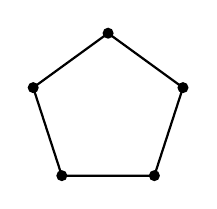
\begin{tikzpicture}
    \coordinate (A) at (90:1);
    \coordinate (B) at (162:1);
    \coordinate (C) at (234:1);
    \coordinate (D) at (306:1);
    \coordinate (E) at (18:1);
    \draw[thick] (A) -- (B) -- (C) -- (D) -- (E) -- cycle;
    \fill (A) circle (2pt);
    \fill (B) circle (2pt);
    \fill (C) circle (2pt);
    \fill (D) circle (2pt);
    \fill (E) circle (2pt);
\end{tikzpicture}
\end{document}